\documentclass[conference]{IEEEtran}
\usepackage{amsmath,amssymb,amsfonts}
\usepackage{graphicx}
\usepackage{booktabs}
\usepackage{cite}
\usepackage{url}
\usepackage{textcomp}
\usepackage{xcolor}
\usepackage{tikz}
\usepackage{pgfplots}
\pgfplotsset{compat=1.18}
\usetikzlibrary{arrows.meta, positioning, shapes.geometric, fit, backgrounds, calc}
\usepackage{hyperref}

\begin{document}

\title{Privacy-Preserving Instruction Tuning of Small
Language Models for Financial Entity Extraction
via DP-QLoRA}

\author{
  \IEEEauthorblockN{Disha Kwatra, Sandesh Jain, Shivansh Katiyar, Gargi Kalia, Dhruv Sanghvi}
 
}

\maketitle

\begin{abstract}
Automated credit underwriting in India depends on analysing UPI and IMPS transaction narrations to construct applicant spending profiles. Extracting the payee name from each narration is the first and most critical step in this pipeline, yet it remains difficult because narration formats vary widely across banks, and the data itself is too sensitive for cloud-based processing. Fine-tuning a language model on such records carries an additional risk: the model may memorise individual spending patterns, which can later be extracted by an adversary with access to the weights.

We present \textbf{DP-QLoRA}, a pipeline that combines Differentially Private Stochastic Gradient Descent (DP-SGD) with Quantized Low-Rank Adaptation to train a Qwen2.5-1.5B model for payee extraction on a single NVIDIA T4 GPU. To make this combination work in practice, we resolve three engineering incompatibilities between the Opacus privacy engine and 4-bit quantized training that, to our knowledge, have not been addressed in prior work. On a dataset of 4{,}382 UPI and IMPS narration--payee pairs, DP-QLoRA achieves an F1 score of \textbf{84.0\%} at a privacy budget of $\varepsilon \approx 2.0$, compared with 89.3\% for the non-private baseline. Error analysis shows that most of the 5.3-point gap manifests as partial rather than catastrophic extraction failures, preserving downstream utility for merchant classification.
\end{abstract}

\begin{IEEEkeywords}
Differential Privacy, QLoRA, Payee Extraction, Small Language Models
\end{IEEEkeywords}

%% -----------------------------------------------------------
\section{Introduction}
\label{sec:intro}

Bank transaction narrations in India are far more than descriptive text. They serve as the backbone of reconciliation, GST audit trails, vendor identity verification, and accounts-receivable tracking~\cite{rbi2025vision}. Each time a UPI or IMPS transfer is executed, the payment system generates a short narration string that encodes the counterparty name, payment rail, and reference identifiers. With monthly UPI transaction volumes exceeding 17~billion by late 2024~\cite{rbi2025vision}, these narrations collectively form the richest behavioural signal available to lenders: a creditor who knows that an applicant pays rent consistently, spends moderately on food delivery, and has no gambling transactions can price credit risk far more accurately than one relying on a bureau score alone.

Unlocking this signal requires a three-step pipeline. First, the raw narration must be parsed to isolate the counterparty, i.e.\ the \emph{payee}. Second, each payee must be classified as a merchant or an individual. Third, merchant-level data is aggregated into a structured spending profile that feeds a credit-risk model. This paper focuses on the first step, payee extraction, because it is the prerequisite for everything downstream and because the narration strings themselves are noisy, unstructured, and formatted differently by every originating bank.

Two operational constraints make standard approaches inadequate. The first is \emph{data sovereignty}. The Reserve Bank of India's data-localisation framework prohibits routing customer financial data through servers outside India, and India's Digital Personal Data Protection Act~2023 (DPDPA) imposes strict obligations on data fiduciaries~\cite{dwork2006calibrating}. Together, these rules eliminate commercial NLP APIs and foreign cloud inference endpoints. The model must therefore run on hardware that a bank can deploy on premise, which in practice means a single commodity GPU server. This constraint, rather than an academic interest in small models, is why we target the 1.5-billion-parameter class.

The second constraint is \emph{training-time privacy}. Fine-tuning a language model on transaction records causes weight memorisation: Carlini et~al.\ demonstrated that individual data points can be extracted from a trained model's weights~\cite{carlini2021extracting}, and Lukas et~al.\ extended this finding specifically to personally identifiable information~\cite{lukas2023pii}. For data governed by the DPDPA and PCI-DSS, empirical resistance to known attacks is insufficient; a formal, mathematically bounded guarantee is required. Differential Privacy (DP)~\cite{dwork2006calibrating} provides exactly such a guarantee.

A natural workaround might be to train on synthetic or LLM-generated data instead of real transactions. However, Akkus et~al.\ show that this approach exacerbates the problem: fine-tuning on generated data increases PII extraction success rates by over 20\% relative to the pre-trained baseline, because the generated text preserves the structural and semantic patterns of the original corpus and amplifies memorisation~\cite{akkus2025}. Consequently, DP applied directly to real data remains the correct solution.

This paper makes three contributions:
\begin{enumerate}
  \item We describe a working DP-QLoRA pipeline for payee extraction that resolves practical incompatibilities between the Opacus DP engine and 4-bit quantized training, an integration that, to our knowledge, has not been demonstrated before.
  \item We characterise the privacy--utility tradeoff across independently trained models at $\varepsilon \in \{1, 2, 4, 8\}$, identifying $\varepsilon \approx 2.0$ as the knee of the curve where tightening the budget further causes disproportionate utility loss.
  \item We provide an empirical privacy audit using eight membership inference attack variants and analyse how privacy-induced degradation affects downstream financial pipeline utility.
\end{enumerate}

The remainder of this paper is organised as follows. Section~\ref{sec:related} reviews related work on parameter-efficient fine-tuning, privacy risks in fine-tuned models, and differentially private training. Section~\ref{sec:method} describes the system design and the engineering fixes required to combine Opacus with QLoRA. Section~\ref{sec:exp} presents the experimental setup, and Section~\ref{sec:results} discusses results. Section~\ref{sec:conclusion} concludes.

%% -----------------------------------------------------------
\section{Related Work}
\label{sec:related}

Our work sits at the intersection of parameter-efficient fine-tuning, privacy-risk analysis of fine-tuned language models, and differentially private training. We review each area below and highlight the gap that motivates our contribution.

\subsection{Parameter-Efficient Fine-Tuning}

Hu et~al.\ introduced Low-Rank Adaptation (LoRA), which decomposes weight updates into low-rank matrices $\Delta W = AB$ where $A \in \mathbb{R}^{d \times r}$ and $B \in \mathbb{R}^{r \times k}$, keeping the pretrained weights frozen~\cite{hu2022lora}. This dramatically reduces the number of trainable parameters (in our configuration, to just 0.56\% of total weights). The reduction matters not only for memory but also for DP noise calibration: because noise is injected proportional to the gradient norm of \emph{trainable} parameters, fewer trainable parameters translate directly into lower noise for the same privacy budget. Dettmers et~al.\ extended this idea with QLoRA, which quantizes the frozen base weights to 4-bit NormalFloat (NF4) while keeping adapters in float16~\cite{qlora}, enabling 1.5B-parameter models to fit within 16\,GB of GPU memory.

\subsection{Privacy Risks in Fine-Tuned Models}

Membership inference attacks (MIAs) were formalised by Shokri et~al.~\cite{shokri2017membership}, who showed that fine-tuning amplifies memorisation: training on a subset of data makes the model more likely to reproduce related records. More recently, Ran et~al.'s LoRA-Leak framework demonstrated that LoRA-tuned models remain vulnerable to MIAs even at conservative training depths, with attack AUC reaching 0.775 on medical QA data after only three epochs~\cite{loraleak}. Furthermore, using the publicly available pretrained model as a calibration reference consistently amplifies attack effectiveness. These empirical findings establish that parameter efficiency alone does not confer privacy. Critically for our setting, Akkus et~al.\ confirmed that training on synthetic data does not mitigate these risks; rather, it exacerbates them~\cite{akkus2025}. These findings collectively motivate the formal DP guarantee we adopt, rather than relying on empirical resistance alone.

\subsection{Differentially Private Fine-Tuning}

Yu et~al.\ established that DP-SGD can be applied to language model fine-tuning at practical utility levels~\cite{yu2022differentially}. Yao et~al.\ combined DP with LoRA for instruction tuning, reporting reduced MIA-AUC with acceptable precision cost~\cite{yao2024dplora}. However, neither work addresses the engineering conflicts introduced by 4-bit quantization. Specifically, combining Opacus with NF4-quantized models produces gradient-hook failures, batch-dimension mismatches, and loss-dilution effects that prevent training from proceeding at all. We resolve these conflicts in Section~\ref{sec:method}, providing what is, to our knowledge, the first demonstration of a working DP-SGD pipeline on 4-bit quantized models with the Opacus framework.

%% -----------------------------------------------------------
\section{System and Methodology}
\label{sec:method}

\subsection{Problem Formulation}

We frame payee extraction as a conditional text-generation task. Given a raw narration string, the model must produce the normalised payee name. Formally, let $\mathcal{D} = \{(x_i, y_i)\}_{i=1}^{N}$ be training pairs where $x_i$ is a raw narration and $y_i$ is the ground-truth payee. We minimise token-level cross-entropy:
\begin{equation}
  \mathcal{L}(\theta) = -\frac{1}{N} \sum_{i=1}^{N} \sum_{t} \log P\!\left(y_i^{(t)} \mid y_i^{(<t)}, x_i;\, \theta\right)
\end{equation}
subject to the constraint that the training procedure satisfies $(\varepsilon, \delta)$-differential privacy. That is, for any two datasets $\mathcal{D}$ and $\mathcal{D}'$ differing by a single record and any output set $\mathcal{S}$:
\begin{equation}
  \Pr[\mathcal{M}(\mathcal{D}) \in \mathcal{S}] \leq e^{\varepsilon} \cdot \Pr[\mathcal{M}(\mathcal{D}') \in \mathcal{S}] + \delta.
\end{equation}
Here, $\varepsilon$ controls the strength of the privacy guarantee (smaller is stricter), and $\delta$ bounds the probability of an outright privacy failure, i.e.\ the chance that the mechanism behaves in a way that cannot be explained by the noise alone.

\subsection{Model Configuration}

We select Qwen2.5-1.5B-Instruct as the base model for two reasons. First, at 1.5~billion parameters, it is large enough to capture the linguistic variation across Indian bank narration formats, yet small enough to fit on a single 16\,GB GPU when quantized. Second, the Qwen2.5 architecture supports the attention-layer LoRA injection points required by our pipeline. The model is quantized to 4-bit NF4 using BitsAndBytes double-quantization with float16 compute dtype, which halves the memory footprint relative to FP16 while preserving most of the model's capacity.

LoRA adapters are injected into the query, key, value, and output projection matrices of all transformer layers with rank $r=16$, scaling factor $\alpha=32$, and dropout $p=0.05$. This yields 8.4M trainable parameters out of 1.5B total (0.56\%), a ratio that is critical for DP: the per-sample noise magnitude scales with the number of trainable parameters, so keeping this fraction small directly reduces the accuracy cost of the privacy guarantee.

Fig.~\ref{fig:pipeline} illustrates the complete training pipeline.
 
%% ── FIGURE 1: Pipeline ────────────────────────────────────────
\begin{figure}[!ht]
\centering
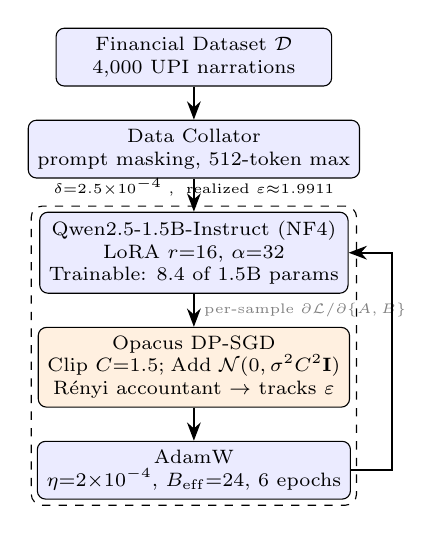
\begin{tikzpicture}[
  node distance=0.42cm and 4.2cm,
  box/.style={draw, rounded corners=3pt, fill=blue!8,
              minimum width=3.5cm, minimum height=0.52cm,
              font=\scriptsize, align=center},
  dpbox/.style={draw, rounded corners=3pt, fill=orange!12,
                minimum width=3.5cm, minimum height=0.52cm,
                font=\scriptsize, align=center},
  arrow/.style={-Stealth, thick},
  ann/.style={font=\tiny, text=gray}
]
\node[box]   (data)   {Financial Dataset $\mathcal{D}$\\
                        4{,}000 UPI narrations};
\node[box,   below=of data]   (coll)   {Data Collator\\
                        prompt masking, 512-token max};
\node[box,   below=of coll]   (model)  {Qwen2.5-1.5B-Instruct (NF4)\\
                        LoRA $r{=}16$, $\alpha{=}32$\\
                        Trainable: 8.4 of 1.5B params};
\node[dpbox, below=of model]  (opacus) {Opacus DP-SGD\\
                        Clip $C{=}1.5$;\;Add
                        $\mathcal{N}(0,\sigma^2 C^2\mathbf{I})$\\
                        R\'enyi accountant
                        $\to$ tracks $\varepsilon$};
\node[box,   below=of opacus] (opt)    {AdamW\\
                        $\eta{=}2{\times}10^{-4}$,
                        $B_{\mathrm{eff}}{=}24$, 6 epochs};
 
\draw[arrow] (data)   -- (coll);
\draw[arrow] (coll)   -- (model);
\draw[arrow] (model)  -- node[right,ann]{per-sample
                         $\partial\mathcal{L}/\partial\{A,B\}$}
                         (opacus);
\draw[arrow] (opacus) -- (opt);
\draw[arrow]
(opt.east) -|
([xshift=0.55cm]model.east)
-- (model.east);
 
\node[draw, dashed, rounded corners=4pt,
      fit=(model)(opacus)(opt), inner sep=2pt,
      label={[font=\tiny]above:
      $\delta{=}2.5{\times}10^{-4}$  ,\;
     realized $\varepsilon{\approx}1.9911$}] {};
\end{tikzpicture}
\caption{DP-QLoRA training pipeline on a single Tesla T4 (15.64\,GB).
Only the 8.4M LoRA adapter parameters receive gradient updates,
reducing sensitivity and required noise magnitude relative to
full-parameter DP-SGD.}
\label{fig:pipeline}
\end{figure}
 
\subsection{DP-SGD Protocol}

The Opacus engine implements DP-SGD as described by Abadi et~al.~\cite{abadi2016deep}. For each mini-batch of size $B=24$, per-sample gradients $g_i$ are first clipped to $\ell_2$ norm $C=1.5$, following the adaptive clipping strategy of Andrew et~al.~\cite{andrew2021differentially}:
\begin{equation}
  \tilde{g}_i = g_i \cdot \min\!\left(1, \frac{C}{\|g_i\|_2}\right)
\end{equation}
Gaussian noise is then added to the clipped aggregate before the optimiser step:
\begin{equation}
  \theta_{t+1} = \theta_t - \eta \left(\frac{1}{B}\sum_i \tilde{g}_i + \mathcal{N}\!\left(0, \frac{\sigma^2 C^2}{B^2}I\right)\right)
\end{equation}
with learning rate $\eta = 2 \times 10^{-4}$. We set the clipping norm to $C=1.5$ based on empirical analysis of gradient norms during preliminary non-private runs; this value clips approximately 60\% of per-sample gradients, balancing signal preservation against sensitivity reduction. Privacy accounting uses R\'{e}nyi Differential Privacy (RDP) composition~\cite{mironov2017renyi}, converted to $(\varepsilon, \delta)$ form with $\delta = 10^{-5}$ after each epoch.

\subsection{Engineering Fixes for Opacus--QLoRA Compatibility}

Combining Opacus with QLoRA on the Qwen2.5 architecture produces three structural failures that must be resolved before training can begin. Each fix addresses a distinct layer of incompatibility between the DP engine's assumptions and the quantized training setup.

\textbf{Gradient checkpointing conflict.} Opacus registers forward-backward hooks on each trainable module to capture per-sample gradients. Gradient checkpointing, which most memory-constrained LLM training pipelines rely on, recomputes activations during the backward pass, invalidating these hooks and producing a \texttt{ValueError} at the optimiser step due to tensor-shape mismatches. Most prior DP fine-tuning work assumes gradient checkpointing is available for memory savings, making its removal counterintuitive. We disable it entirely and compensate by truncating sequences to 64 tokens; with only 0.56\% of parameters trainable, the full computation graph fits within 16\,GB without checkpointing.

\textbf{Poisson sampling conflict.} DP accounting theory assumes Poisson subsampling of the training set, which produces variable-size batches. In practice, these variable dimensions cause shape mismatches in the quantized NF4 matrix multiplications that underlie the frozen base weights. We disable Poisson sampling (\texttt{poisson\_sampling=False}) and use fixed shuffled batches instead. The RDP accountant correctly tracks privacy composition under this fixed-batch regime, yielding a valid but slightly looser bound than ideal Poisson subsampling would provide.

\textbf{Loss dilution from prompt tokens.} By default, the cross-entropy loss is computed over the entire input--output sequence, including the instruction-prompt prefix. Because prompt tokens are identical across samples, they contribute a near-constant gradient that dilutes the payee-specific learning signal. Without correction, the model would require more training epochs to learn the same extraction behaviour, which in turn consumes more of the privacy budget (higher~$\varepsilon$). Our custom data collator masks all prompt token positions with the ignore index (\texttt{-100}), ensuring that loss and gradients are derived exclusively from the target payee tokens. This fix is therefore not just accuracy-enhancing but also privacy-enhancing: it reduces the number of epochs needed to reach a given utility level.

%% -----------------------------------------------------------
\section{Experiments}
\label{sec:exp}

\subsection{Dataset and Setup}

The training set comprises 4{,}382 UPI and IMPS narration--payee pairs, manually annotated from transaction records spanning P2P transfers, merchant payments, and utility credits across multiple originating banks and payment rails. A separate set of 486 pairs is held out for validation. Narration formats vary substantially: some banks include the beneficiary name in a fixed field, others embed it within a free-text description alongside reference numbers, and still others truncate or abbreviate names unpredictably. No personally identifiable information is retained in any released artefact; all payee labels are normalised to merchant or individual names without associated account numbers.

All experiments run on a single NVIDIA T4 GPU with 15.64\,GB of memory. The optimiser is AdamW with a learning rate of $2 \times 10^{-4}$, and training runs for six epochs.

We compare DP-QLoRA against four baselines: zero-shot Qwen2.5-1.5B, zero-shot Llama-3.2-1B-Instruct, zero-shot Gemma-2-2B-IT, and non-private QLoRA (identical configuration to DP-QLoRA but without the DP-SGD wrapper). All baselines use the same prompt format and evaluation set.

The primary utility metric is token-level F1, computed by aligning predicted and ground-truth payee strings at the character level. We also report exact match (after character normalisation) and token-level precision and recall. For privacy evaluation, we run eight membership inference attack (MIA) variants and report MIA-AUC.

\begin{table*}[!ht]
\caption{Extraction Performance on Sample Test Set}
\label{tab:perf}
\centering
\begin{tabular}{@{}lcccc@{}}
\toprule
\textbf{Model} &
\textbf{Exact Match (\%)} &
\textbf{Precision (\%)} &
\textbf{Recall (\%)} &
\textbf{F1 Score (\%)} \\
\midrule
Base Qwen2.5-1.5B (0-shot) & 35.4 & 55.9 & 62.1 & 57.5 \\
Llama-3.2-1B (Meta)        & 55.6 & 66.3 & 67.2 & 66.5 \\
Gemma-2-2B (Google)        & 10.7 & 11.3 & 11.4 & 11.3 \\
QLoRA (non-private)        & 86.2 & 89.4 & 89.3 & 89.3 \\
\textbf{DP-QLoRA ($\varepsilon{\approx}2.0$)} &
\textbf{62.8} &
\textbf{80.4} &
\textbf{89.8} &
\textbf{84.0} \\
\bottomrule
\end{tabular}
\end{table*}


%% -----------------------------------------------------------
\section{Results}
\label{sec:results}

\subsection{Extraction Performance}

Table~\ref{tab:perf} summarises extraction performance across all models. DP-QLoRA at $\varepsilon \approx 2.0$ achieves an F1 of 84.0\%, outperforming every zero-shot baseline, including Llama-3.2-1B at 66.5\%, while providing a formal privacy guarantee that none of the baselines offer. The non-private QLoRA ceiling stands at 89.3\%, so the cost of differential privacy is 5.3~F1 points. Fig.~\ref{fig:accuracy} presents the full metric breakdown.

\begin{figure}[!ht]
  \centering
  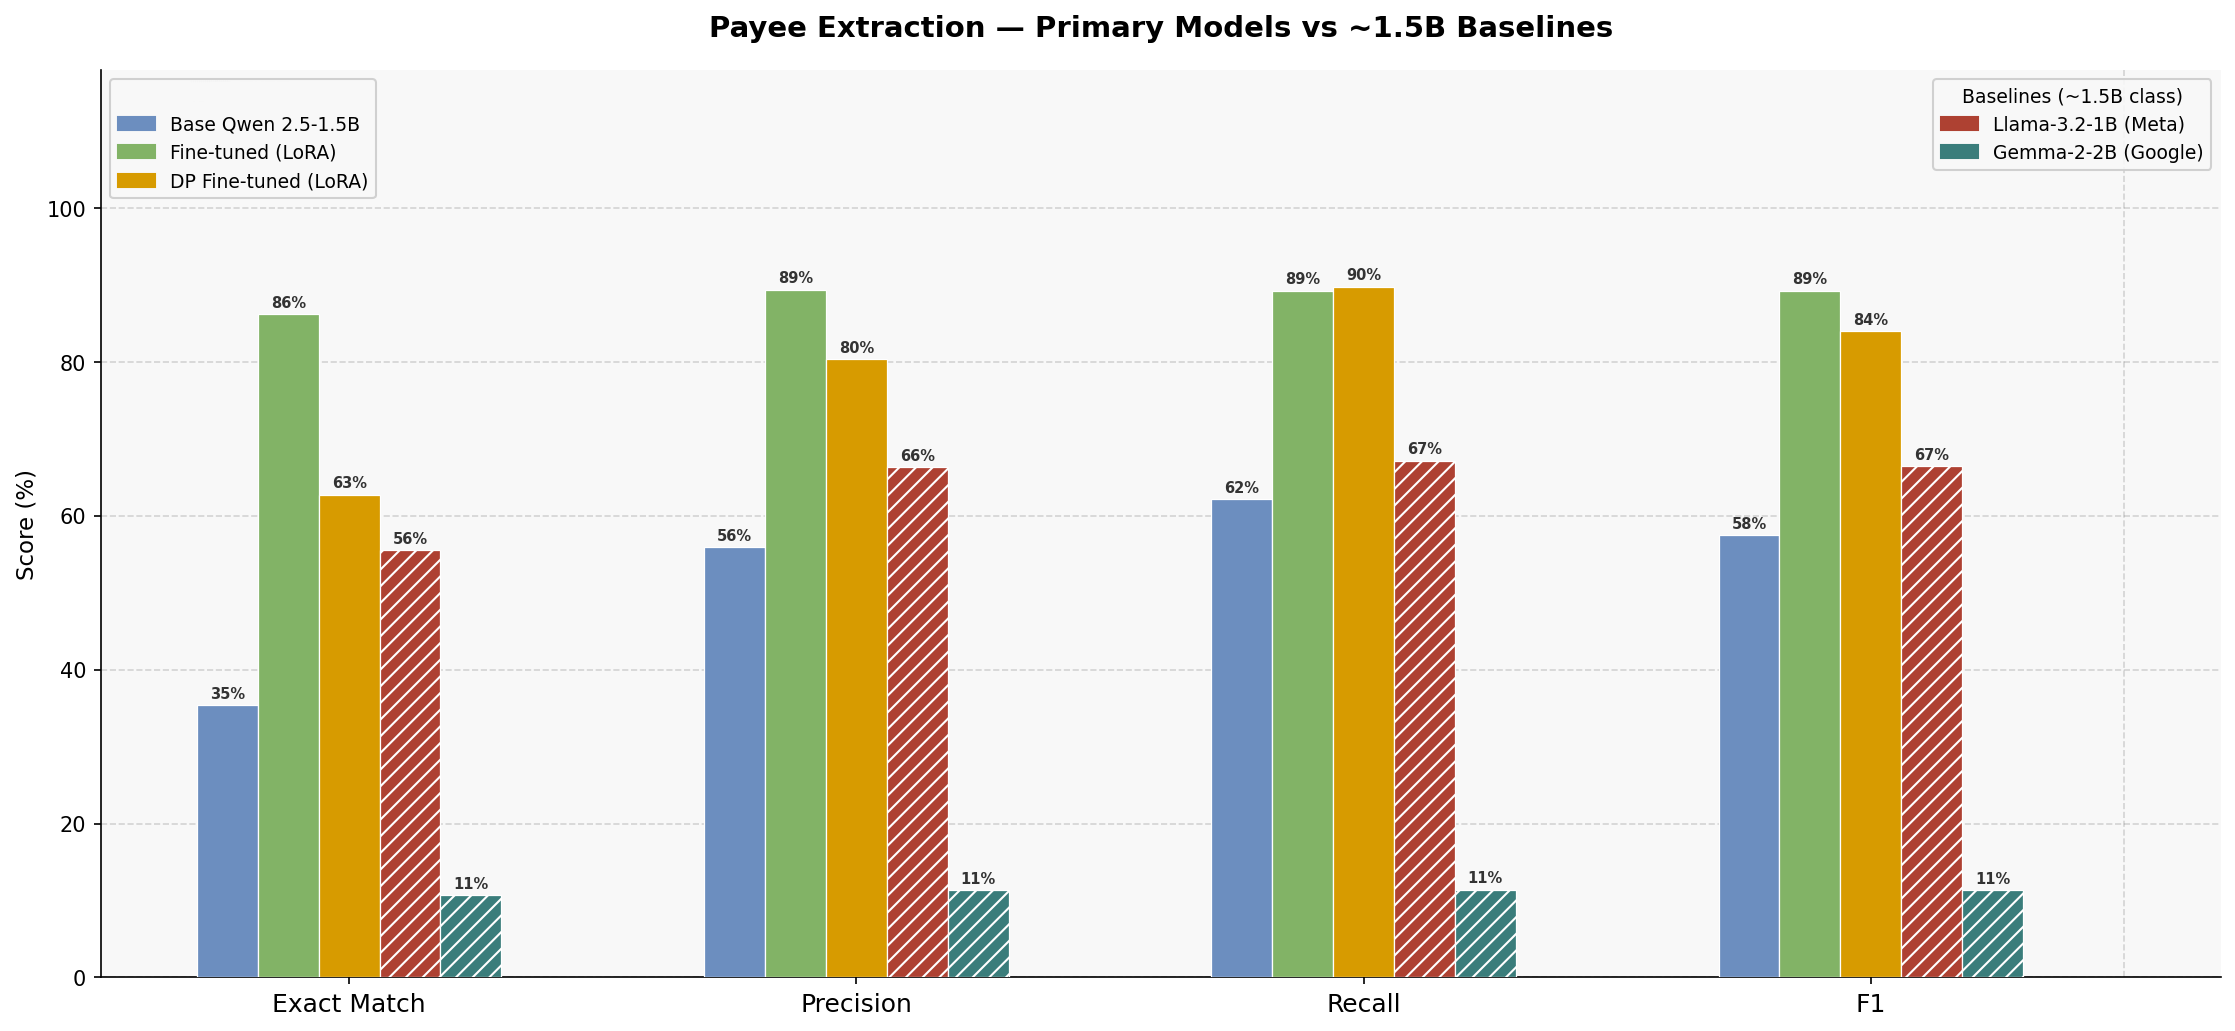
\includegraphics[width=\columnwidth]{plots/graph1_accuracy_all_models.png}
  \caption{Extraction performance across all models and metrics. DP Fine-tuned (LoRA) refers to DP-QLoRA at $\varepsilon \approx 2.0$.}
  \label{fig:accuracy}
\end{figure}

A closer look at the precision--recall split reveals a telling pattern. The recall of DP-QLoRA (89.8\%) nearly matches the non-private model (89.3\%), whereas precision drops more noticeably (80.4\% vs.\ 89.4\%). This asymmetry is consistent with DP noise broadening the model's output distribution: the model correctly identifies the payee token region but is less precise about exact capitalisation, spacing, and boundary characters.

Fig.~\ref{fig:errors} confirms this interpretation through the error breakdown. The privacy cost appears almost entirely as a shift from exact matches (85.2\%$\to$61.7\%) to partial matches (7.2\%$\to$29.2\%), while complete extraction failures increase only marginally (7.6\%$\to$9.1\%). Gemma-2-2B's notably low performance (11.3\% F1) is attributable to its instruction-following format being poorly suited to the structured extraction prompt: it frequently generated verbose explanations rather than isolated payee names, causing both precision and recall to collapse. For the downstream merchant classification task, partial matches (where the payee name is recognisably correct but includes minor formatting artefacts) are recoverable through string normalisation.

\begin{figure}[!ht]
  \centering
  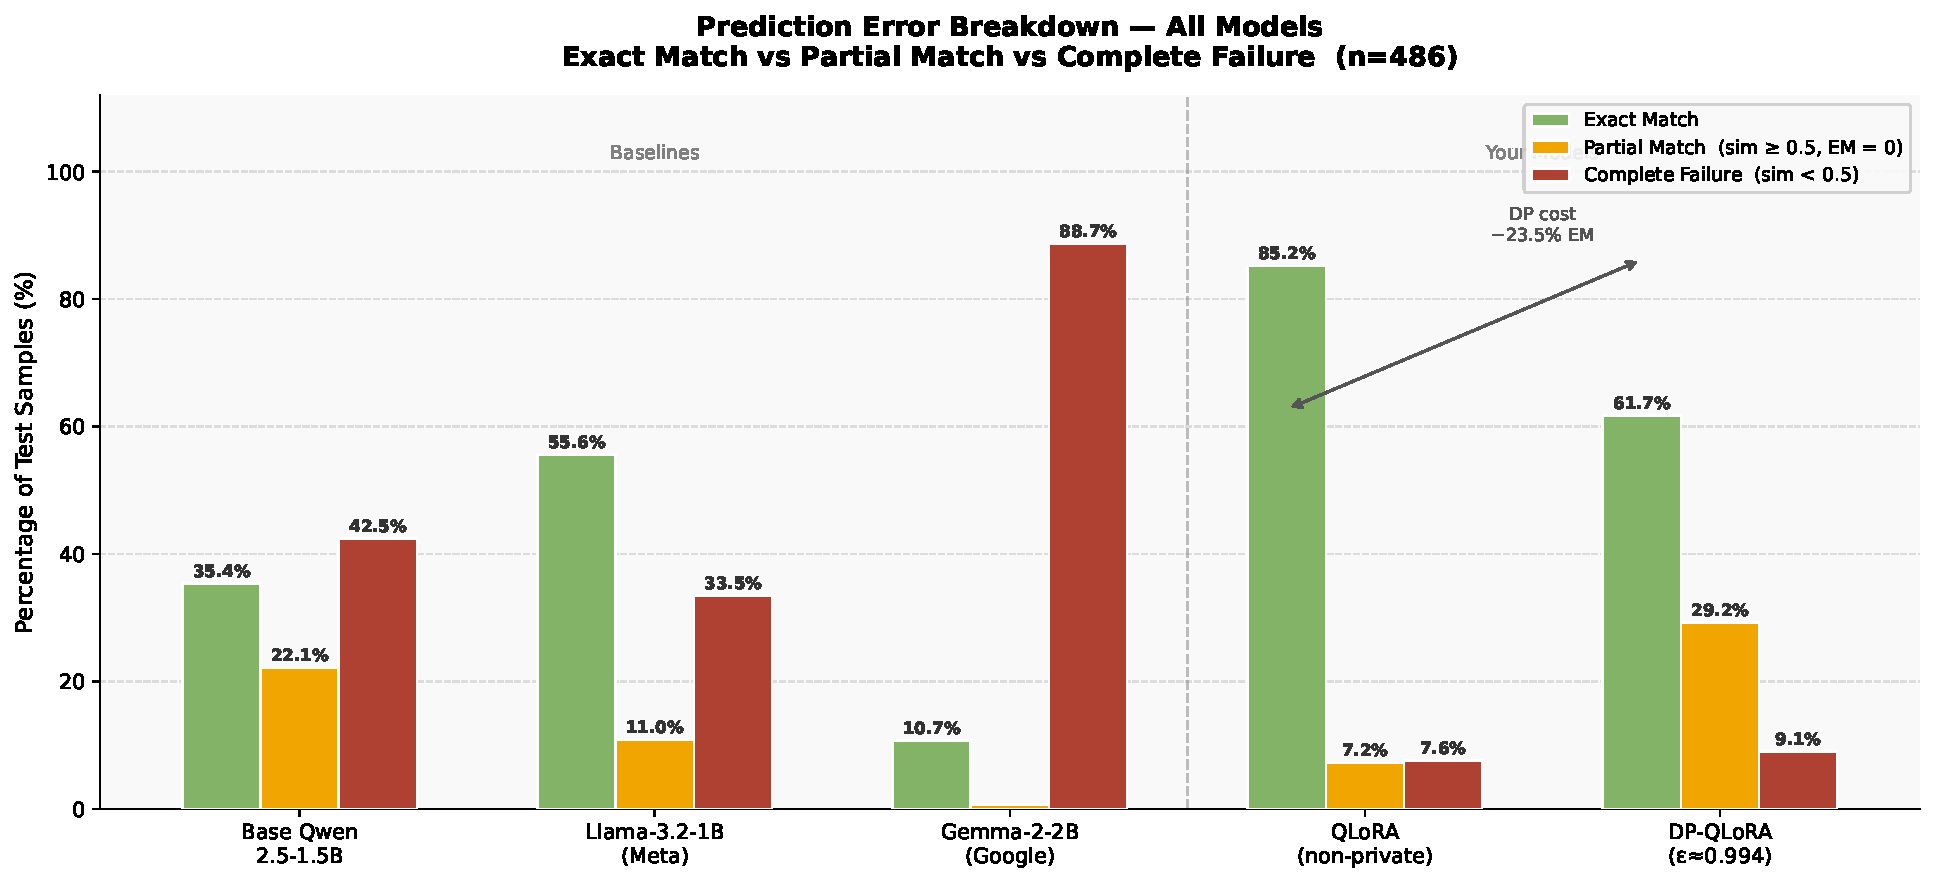
\includegraphics[width=\columnwidth]{plots/fig2b_error_breakdown.pdf}
  \caption{Error breakdown by category. The DP cost of $-23.5\%$ exact match converts almost entirely to partial matches rather than catastrophic failures, preserving downstream pipeline utility.}
  \label{fig:errors}
\end{figure}

\subsection{Training Dynamics}

Having established DP-QLoRA's extraction quality, we now examine its training behaviour to understand how gradient noise affects convergence.

Fig.~\ref{fig:loss} shows the loss curves for both configurations. Non-private QLoRA converges to a validation loss of 0.03 within two epochs, exhibiting clean generalisation with minimal overfitting. DP-QLoRA, by contrast, converges more slowly due to the injected gradient noise, stabilising around a validation loss of 0.62 by epoch~6. The $\varepsilon$ annotations on the DP training curve trace the privacy budget as it accumulates under RDP composition: from 1.29 at epoch~1 to 1.99 at epoch~6. The gap between the two validation losses (0.03 vs.\ 0.62) reflects the fundamental tension between privacy and learning: the noise that prevents memorisation also slows convergence and limits the achievable loss floor.

\begin{figure}[!ht]
  \centering
  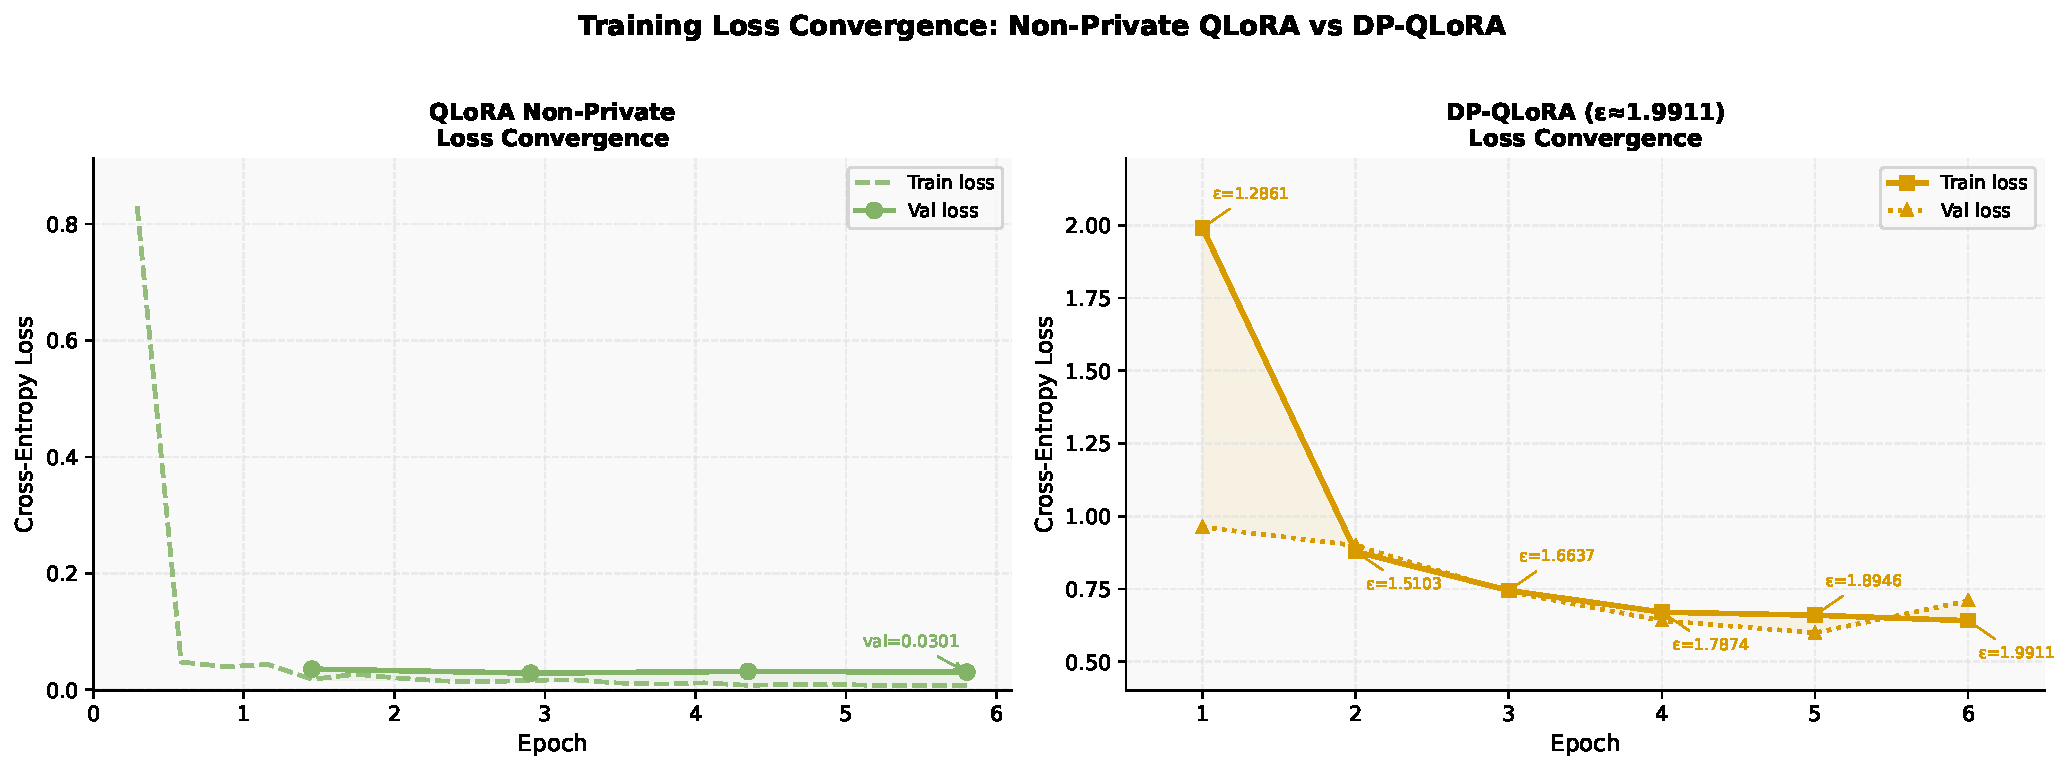
\includegraphics[width=\columnwidth]{plots/fig1_loss_convergence.pdf}
  \caption{Training and validation loss convergence. Left: non-private QLoRA reaches val.\ loss 0.03. Right: DP-QLoRA stabilises near 0.62 with per-epoch $\varepsilon$ annotated on the training curve.}
  \label{fig:loss}
\end{figure}

\subsection{Privacy--Utility Tradeoff}

To map the tradeoff between privacy strength and extraction quality, we train four independent DP-QLoRA models at $\varepsilon \in \{1, 2, 4, 8\}$. Each model is trained from scratch with a fixed privacy budget, so utility differences are attributable to the privacy constraint rather than training duration. We use character-level similarity as a per-sample proxy for F1; unlike token-level F1, character similarity is tokenizer-agnostic and avoids introducing evaluation artefacts from subword segmentation differences across models.

Fig.~\ref{fig:tradeoff} shows the result. Character similarity rises steeply from 0.785 at $\varepsilon=1$ to 0.841 at $\varepsilon=2$, then plateaus between $\varepsilon=2$ and $\varepsilon=4$ (both 0.841). This plateau confirms that $\varepsilon \approx 2.0$ is the knee of the curve: further relaxing the privacy budget yields diminishing returns in utility while providing a weaker formal guarantee.

\begin{figure}[!ht]
  \centering
  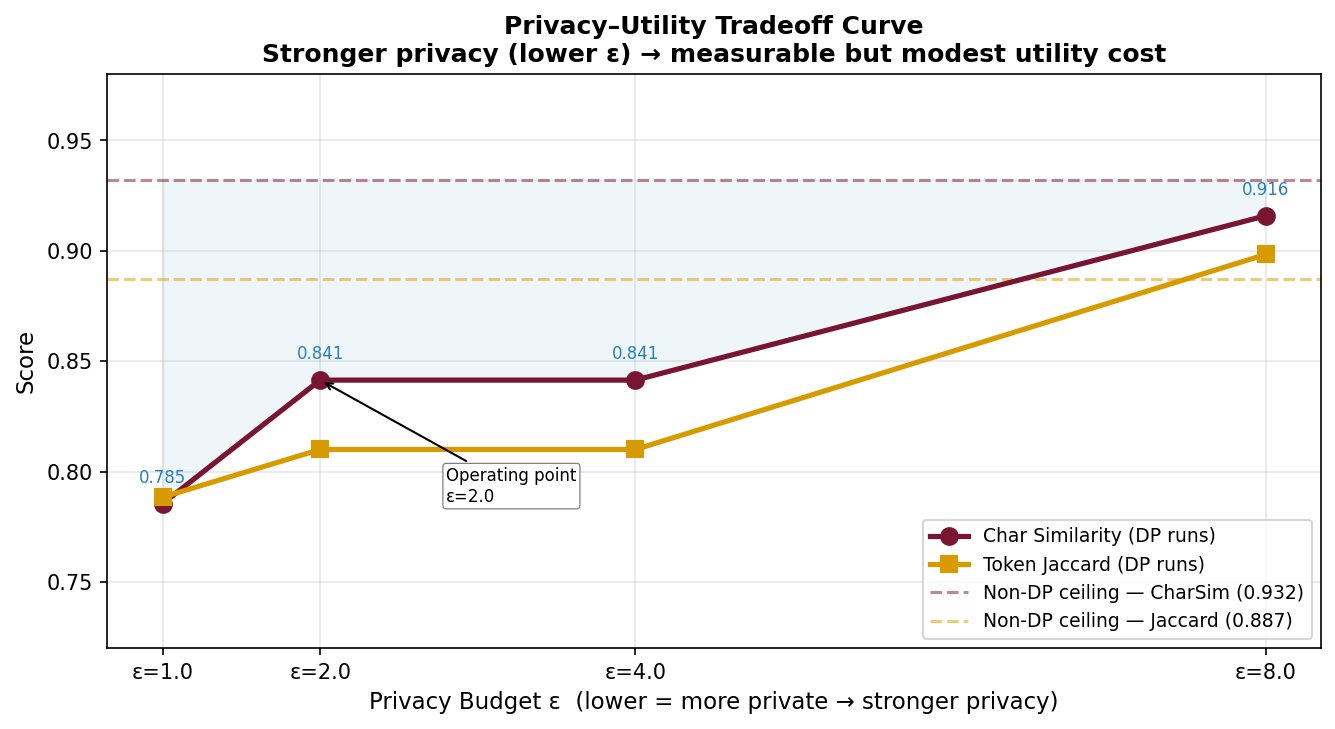
\includegraphics[width=\columnwidth]{plots/privacy_utility.png}
  \caption{Privacy--utility tradeoff from independently trained DP-QLoRA 
models at $\varepsilon \in \{1, 2, 4, 8\}$. Each point is a separate 
training run. The operating point ($\varepsilon{\approx}2.0$, char.\ similarity$=$0.841) 
sits at the knee of the curve.}
  \label{fig:tradeoff}
\end{figure}

From a deployment perspective, a bank seeking stricter privacy should expect character similarity near 0.785 at $\varepsilon=1$, which remains within an acceptable utility band for downstream merchant classification after normalisation.

\subsection{Privacy Audit}

Finally, we evaluate the empirical privacy posture of the $\varepsilon \approx 2.0$ model through membership inference attacks. Fig.~\ref{fig:mia} summarises MIA performance across eight attack variants, including Min-K\% probability and pretrained-calibrated attacks following the LoRA-Leak framework~\cite{loraleak}. All AUC values remain close to random guessing ($0.487$--$0.552$), indicating limited observable memorisation under the evaluated threat model.

We emphasise, however, that empirical MIA audits are inherently incomplete: they evaluate resistance against \emph{specific} attack implementations, and adaptive adversaries may develop stronger strategies over time. For this reason, we treat the formal $(\varepsilon, \delta)$-DP guarantee as the primary privacy mechanism and the MIA audit as complementary empirical evidence~\cite{duan2024mia}.

\begin{figure}[!ht]
\centering
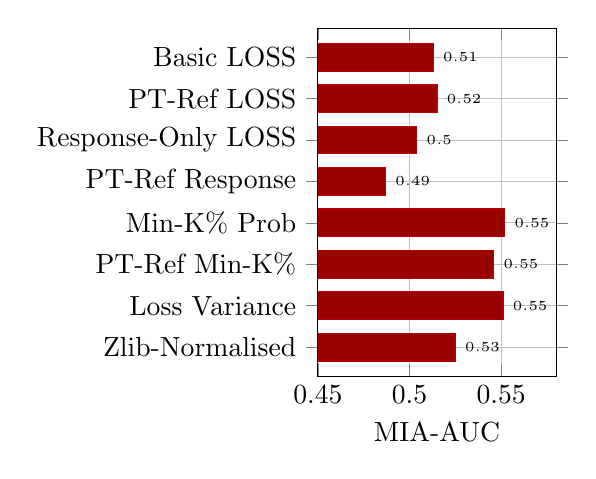
\begin{tikzpicture}
\begin{axis}[
    xbar,
    width=0.38\textwidth,,
    height=6cm,
    xmin=0.45, xmax=0.58,
    xlabel={MIA-AUC},
    symbolic y coords={
        Basic LOSS,
        PT-Ref LOSS,
        Response-Only LOSS,
        PT-Ref Response,
        Min-K\% Prob,
        PT-Ref Min-K\%,
        Loss Variance,
        Zlib-Normalised
    },
    ytick=data,
    y dir=reverse,
    grid=major,
    nodes near coords,
    every node near coord/.append style={
        font=\tiny %5
    },
]

\addplot 
[   fill=red!60!black,
    draw=red!70!black
] coordinates{
(0.513,{Basic LOSS})
(0.515,{PT-Ref LOSS})
(0.504,{Response-Only LOSS})
(0.487,{PT-Ref Response})
(0.552,{Min-K\% Prob})
(0.546,{PT-Ref Min-K\%})
(0.551,{Loss Variance})
(0.525,{Zlib-Normalised})
};

\end{axis}
\end{tikzpicture}

\caption{Membership inference attack AUC across eight attack variants for DP-QLoRA ($\varepsilon \approx 2.0$). All attacks remain near the random baseline ($0.50$), indicating limited observable memorisation.}
\label{fig:mia}
\end{figure}

%% -----------------------------------------------------------
\section{Conclusion}
\label{sec:conclusion}

We have presented DP-QLoRA, a system for extracting payee names from Indian banking transaction narrations under joint hardware and privacy constraints. By resolving three engineering incompatibilities between Opacus and 4-bit quantized training, the system achieves an F1 of 84.0\% at $\varepsilon \approx 2.0$ on a single NVIDIA T4 GPU, within 5.3 points of the non-private ceiling, while providing a formal $(\varepsilon, \delta)$-DP guarantee.

Two findings are particularly relevant for practitioners. First, the privacy cost is concentrated in partial-match errors rather than complete extraction failures, meaning that downstream pipeline stages (merchant classification, spending-profile construction) remain largely unaffected after string normalisation. Second, the privacy--utility tradeoff plateaus at $\varepsilon \approx 2.0$, giving deployers a clear operating point: tightening the budget further to $\varepsilon = 1$ reduces character similarity by approximately 5.6 percentage points, while relaxing it to $\varepsilon = 8$ yields no measurable improvement.

Future work will investigate generalisation across public-sector bank narration formats, which use different field conventions from the private-sector statements in our current dataset. We also plan to evaluate stronger adaptive privacy attacks and extend the framework to multilingual and mixed-script transaction descriptions common in Indian banking.

\begin{thebibliography}{99}

\bibitem{rbi2025vision}
Reserve Bank of India, ``Payment Systems Vision 2025,'' RBI, Mumbai, 2022. [Online]. Available: \url{https://www.rbi.org.in}

\bibitem{carlini2021extracting}
N.~Carlini et al., ``Extracting training data from large language models,'' in \textit{Proc.\ USENIX Security}, 2021, pp.~2633--2650.

\bibitem{lukas2023pii}
N.~Lukas et al., ``Analyzing leakage of personally identifiable information in language models,'' in \textit{Proc.\ IEEE S\&P}, 2023.

\bibitem{dwork2006calibrating}
C.~Dwork, F.~McSherry, K.~Nissim, and A.~Smith, ``Calibrating noise to sensitivity in private data analysis,'' in \textit{Proc.\ TCC}, 2006, pp.~265--284.

\bibitem{akkus2025}
A.~Akkus et al., ``Generated data with fake privacy: Hidden dangers of fine-tuning large language models on generated data,'' in \textit{Proc.\ USENIX Security}, 2025.

\bibitem{hu2022lora}
E.~J.~Hu et al., ``LoRA: Low-rank adaptation of large language models,'' in \textit{Proc.\ ICLR}, 2022.

\bibitem{qlora}
T.~Dettmers, A.~Pagnoni, A.~Holtzman, and L.~Zettlemoyer, ``QLoRA: Efficient finetuning of quantized LLMs,'' in \textit{Proc.\ NeurIPS}, 2023.

\bibitem{shokri2017membership}
R.~Shokri, M.~Stronati, C.~Song, and V.~Shmatikov, ``Membership inference attacks against machine learning models,'' in \textit{Proc.\ IEEE S\&P}, 2017.

\bibitem{loraleak}
D.~Ran, X.~He, T.~Cong, A.~Wang, Q.~Li, and X.~Wang, ``LoRA-Leak: Membership inference attacks against LoRA fine-tuned language models,'' \textit{arXiv:2507.18302}, 2025.

\bibitem{yu2022differentially}
D.~Yu et al., ``Differentially private fine-tuning of language models,'' in \textit{Proc.\ ICLR}, 2022.

\bibitem{yao2024dplora}
G.~Yao, ``Privacy-preserving low-rank instruction tuning for large language models via DP-LoRA,'' \textit{J.\ Comput.\ Technol.\ Softw.}, vol.~3, no.~5, 2024.

\bibitem{abadi2016deep}
M.~Abadi et al., ``Deep learning with differential privacy,'' in \textit{Proc.\ ACM CCS}, 2016, pp.~308--318.

\bibitem{andrew2021differentially}
G.~Andrew, O.~Thakkar, B.~McMahan, and S.~Ramaswamy, ``Differentially private learning with adaptive clipping,'' in \textit{Proc.\ NeurIPS}, 2021.

\bibitem{duan2024mia}
M.~Duan et al., ``Do membership inference attacks work on large language models?'' \textit{arXiv:2402.07841}, 2024.

\bibitem{mironov2017renyi}
I.~Mironov, ``R\'{e}nyi differential privacy,'' in \textit{Proc.\ IEEE CSF}, 2017, pp.~263--275.

\bibitem{tirumala2022memorization}
K.~Tirumala et al., ``Memorization without overfitting: Analyzing the training dynamics of large language models,'' in \textit{Proc.\ NeurIPS}, 2022.

\end{thebibliography}

\end{document}
